% motivation
\graphicspath{{images/motivation/}}
\section{Motivation}
\begin{frame}
	\frametitle{Motivation}
	Bipedal walking is difficult activity to describe due to nonlinear relationships.
	\begin{columns}
	\begin{column}{0.35\textwidth}
		\begin{figure}
		\begin{overprint}
			\onslide<1>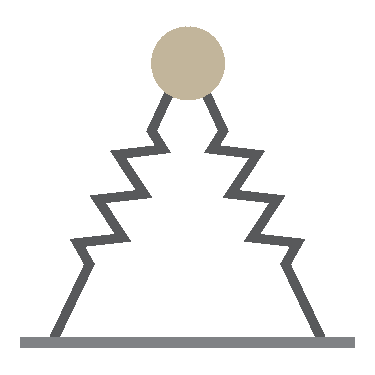
\includegraphics[width=.9\textwidth]{double_SLIP.pdf}
			\onslide<2>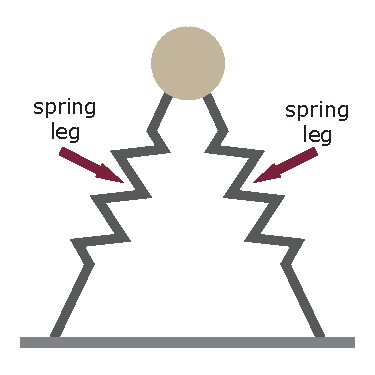
\includegraphics[width=.9\textwidth]{double_SLIP_spring_leg.pdf}
			\onslide<3>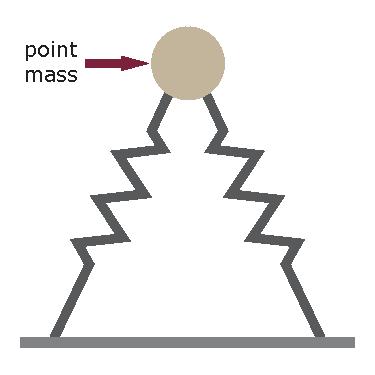
\includegraphics[width=.9\textwidth]{double_SLIP_mass.pdf}
			\onslide<4->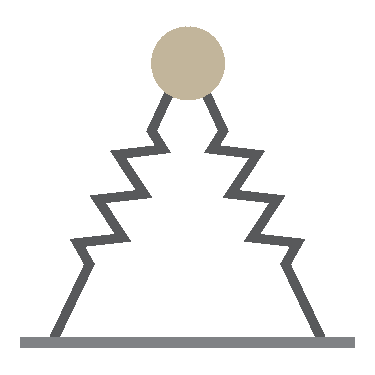
\includegraphics[width=.9\textwidth]{double_SLIP.pdf}		
		\end{overprint}			
		\caption{Spring-loaded inverted pendulum}
	\end{figure}
	\end{column}
	\begin{column}{0.65\textwidth}
	\begin{itemize}
		\item Physical representation of legs as springs \footnotemark[1] \\[1em]
		\item Motion of the trunk with center of mass\footnotemark[1] \\[1em]
		\item Recent works perform bipedal walking with machine learning methods\footnotemark[2]\textsuperscript{,}\footnotemark[3] \\[1em]	
		\item Deep reinforcement learning (DRL) does not require mathematical model or control formulation\footnotemark[4]
		\item DRL with proximal policy optimization is simple and efficient\footnotemark[4]
	\end{itemize}
	\end{column}	
	\end{columns}
	
	\footnotetext[1]{H. Geyer (2006).}
	\footnotetext[2]{T. Haarjona (2019).}
	\footnotetext[3]{T. Li (2019).}
	\footnotetext[4]{J. Schulman (2017)}
	
\end{frame}